\section{Especificación de Requerimientos}
\label{sc:ER}

Este sistema tiene como propósito apoyar al personal clínico en la estimación automática del estadio de heridas ulcerosas en pacientes con pie diabético, utilizando imágenes médicas procesadas mediante técnicas de segmentación, extracción de características radiómicas y modelos de predicción basados en aprendizaje automático.


\subsection{Requerimientos Funcionales}
\label{ssc:RF}

\begin{itemize}
    \item \textbf{RF1: Registro de usuario.} El sistema debe permitir registrar nuevos usuarios en la tabla \texttt{user}, incluyendo su RUT, nombre, correo, contraseña, rol y fecha de nacimiento.

    \item \textbf{RF2: Gestión de pacientes.} El sistema debe permitir al personal clínico registrar y actualizar información de pacientes en la tabla \texttt{paciente}, asociando cada paciente a un usuario y a un profesional responsable.

    \item \textbf{RF3: Registro de profesionales.} El sistema debe permitir registrar y administrar profesionales clínicos en la tabla \texttt{profesional}, vinculando cada uno a un usuario registrado.

    \item \textbf{RF4: Carga de imágenes clínicas.} El sistema debe permitir subir imágenes de heridas ulcerosas, guardando su nombre, fecha de captura, ruta de almacenamiento y asociación con el paciente correspondiente en la tabla \texttt{imagen}.

    \item \textbf{RF5: Segmentación de imágenes.} El sistema debe permitir registrar los resultados de segmentación de una imagen, especificando el método usado (manual o automática), la ruta de la máscara y la fecha de creación, en la tabla \texttt{segmentacion}.

    \item \textbf{RF6: Evaluación del estadio de la herida.} El sistema debe permitir registrar el puntaje PWAT calculado por modelo o experto humano en la tabla \texttt{pwatscore}, vinculando los resultados con una imagen y su segmentación correspondiente.

    \item \textbf{RF7: Visualización de evaluaciones.} El sistema debe permitir consultar el historial de evaluaciones PWAT asociadas a un paciente, visualizando fecha, evaluador, observaciones, imagen relacionada y resultados por categoría (JSON).

    \item \textbf{RF8: Validación cruzada de evaluaciones.} El sistema debe permitir comparar las evaluaciones realizadas por el modelo con aquellas realizadas por expertos clínicos sobre la misma imagen.

    \item \textbf{RF9: Gestión de acceso por rol.} El sistema debe restringir el acceso a funcionalidades según el campo \texttt{rol} de la tabla \texttt{user}, permitiendo, por ejemplo, que sólo usuarios con rol \texttt{doctor} o \texttt{enfermera} puedan ingresar evaluaciones clínicas.

\end{itemize}



\subsection{Requerimientos No Funcionales}
\label{ssc:RNF}

\begin{itemize}
    \item \textbf{RNF1:} El sistema debe procesar una imagen y mostrar el resultado en un tiempo máximo de 5 segundos.
    
    \item \textbf{RNF2:} El sistema debe ser portable y permitir escalabilidad horizontal mediante contenedores Docker, de forma que se puedan ejecutar multiples instancias concurrentes
    
    \item \textbf{RNF3:} El sistema debe tener una disponibilidad mínima del 99.5\% mensual.
    
    \item \textbf{RNF4:} El sistema debe utilizar cifrado TLS 1.2 o superior para la transmisión de imágenes y datos clínicos.
    
    \item \textbf{RNF5:} La interfaz de usuario debe ser intuitiva y responsiva, compatible con dispositivos móviles y navegadores modernos.
    
    \item \textbf{RNF6:} El código del sistema debe estar modularizado y documentado, facilitando su mantenimiento evolutivo y correctivo.
    
    \item \textbf{RNF7:} El sistema debe ser compatible con las tres últimas versiones de los navegadores Chrome, Firefox, Safari y Edge.
    
    \item \textbf{RNF8:} El backend debe permitir la interoperabilidad entre servicios desarrollados en Node.js y scripts Python, mediante APIs REST o invocaciones asincrónicas.
    
    \item \textbf{RNF9:} Cada predicción debe ser registrada con un identificador único y metadatos asociados (timestamp, parámetros utilizados, resultado) para permitir trazabilidad clínica y técnica.
\end{itemize}


\section{Funcionalidades del Sistema}
\label{sc:FS}


\subsection{Diagramas de Casos de Uso}
\label{ssc:DCU}

\begin{figure}[H] %si cambia la "H" por "t", se fuerza a que la figura quede arriba de la página
    \centering
    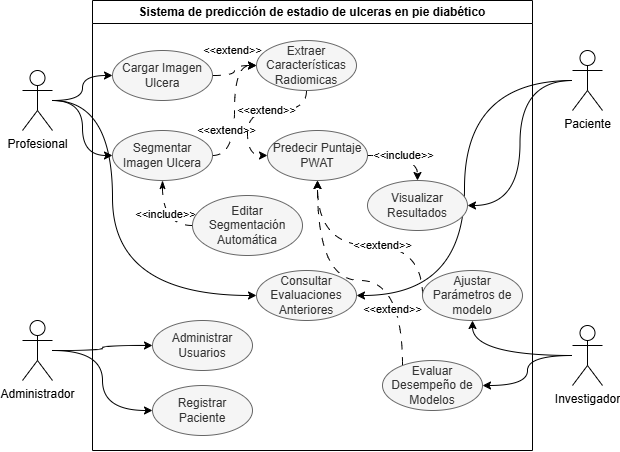
\includegraphics[width=1.1\textwidth]{imagenes/casosdeuso.drawio.png}
    \caption{Diagrama de casos de uso}
    \label{fig:scrum}
\end{figure}


\subsection{Casos de Uso (resumidos)}
\label{ssc:CUresumido}

\begin{table}[H]
  \small
  \centering
  \caption{Resumen condensado de Casos de Uso}
  \label{tab:cu_resumido}
  \begin{tabular}{p{1cm} p{6cm} p{2cm} p{4cm}}
    \toprule
    \textbf{ID} & \textbf{Descripción}                          & \textbf{Actor(es)}           & \textbf{Relación}           \\
    \midrule
    CU01        & Carga imagen de la úlcera                     & Profesional                  & Extiende CU02               \\
    CU02        & Extrae características radiomédicas           & Profesional                  & Depende de CU01             \\
    CU03        & Segmenta la imagen de la úlcera               & Profesional                  & Depende de CU01             \\
    CU04        & Edita segmentación automática                 & Profesional                  & Extiende CU03               \\
    CU05        & Visualiza resultados (PWAT)                   & Profesional, Paciente        & Incluye CU03, CU06          \\
    CU06        & Calcula y guarda puntaje PWAT                 & Profesional                  & Depende de CU03             \\
    CU07        & Consulta historial de evaluaciones            & Profesional, Paciente        & Depende de CU06             \\
    CU08        & Gestiona registro de paciente                 & Administrador                & –                           \\
    CU09        & Gestiona usuarios                             & Administrador                & –                           \\
    CU10        & Ajusta parámetros del modelo predictivo       & Investigador                 & Depende de CU06             \\
    CU11        & Evalúa desempeño del modelo                   & Investigador                 & Depende de CU06             \\
    \bottomrule
  \end{tabular}
\end{table}



\subsection{Especificación de Casos de Uso}
\label{ssc:CUEspec}

\paragraph{CU01 -- Cargar Imagen Úlcera}
\begin{itemize}
  \item \textbf{Descripción:} Permite al profesional subir o capturar la fotografía clínica de la herida ulcerosa.
  \item \textbf{Actor(es):} Profesional
  \item \textbf{Dependencias:} — (caso de uso inicial)
\end{itemize}

\paragraph{CU02 -- Extraer Características Radiomédicas}
\begin{itemize}
  \item \textbf{Descripción:} Calcula automáticamente descriptores de textura, forma y color sobre la región segmentada de la herida (radiomics).
  \item \textbf{Actor(es):} Profesional
  \item \textbf{Depende de:} CU01
\end{itemize}

\paragraph{CU03 -- Segmentar Imagen Úlcera}
\begin{itemize}
  \item \textbf{Descripción:} Genera automáticamente las máscaras que delimitan la herida y los diferentes tejidos (granulación, necrosis, epitelización).
  \item \textbf{Actor(es):} Profesional
  \item \textbf{Depende de:} CU01
\end{itemize}

\paragraph{CU04 -- Editar Segmentación Automática}
\begin{itemize}
  \item \textbf{Descripción:} Permite al profesional corregir manualmente cualquier imprecisión en las máscaras obtenidas automáticamente.
  \item \textbf{Actor(es):} Profesional
  \item \textbf{Extiende a:} CU03
\end{itemize}

\paragraph{CU05 -- Visualizar Resultados (PWAT)}
\begin{itemize}
  \item \textbf{Descripción:} Muestra al profesional y al paciente la imagen original, las máscaras de segmentación, los valores de radiomics y el puntaje PWAT calculado.
  \item \textbf{Actor(es):} Profesional, Paciente
  \item \textbf{Incluye:} CU03, CU06
\end{itemize}

\paragraph{CU06 -- Predecir Puntaje PWAT}
\begin{itemize}
  \item \textbf{Descripción:} Invoca el modelo predictor para calcular y almacenar el puntaje PWAT sobre la imagen segmentada.
  \item \textbf{Actor(es):} Profesional
  \item \textbf{Depende de:} CU03
\end{itemize}

\paragraph{CU07 -- Consultar Evaluaciones Anteriores}
\begin{itemize}
  \item \textbf{Descripción:} Permite revisar el historial completo de puntajes PWAT asociados a un paciente o a una imagen concreta.
  \item \textbf{Actor(es):} Profesional, Paciente
  \item \textbf{Depende de:} CU06
\end{itemize}

\paragraph{CU08 -- Registrar Paciente}
\begin{itemize}
  \item \textbf{Descripción:} Crea o actualiza el expediente de un paciente en la base de datos (\texttt{paciente}).
  \item \textbf{Actor(es):} Administrador
  \item \textbf{Dependencias:} — (caso de uso independiente)
\end{itemize}

\paragraph{CU09 -- Administrar Usuarios}
\begin{itemize}
  \item \textbf{Descripción:} Permite dar de alta, baja, modificar y consultar usuarios (profesionales o investigadores) en la tabla \texttt{user}.
  \item \textbf{Actor(es):} Administrador
  \item \textbf{Dependencias:} — (caso de uso independiente)
\end{itemize}

\paragraph{CU10 -- Ajustar Parámetros de Modelos}
\begin{itemize}
  \item \textbf{Descripción:} Permite al investigador reentrenar el modelo de predicción o ajustar sus hiperparámetros.
  \item \textbf{Actor(es):} Investigador
  \item \textbf{Depende de:} CU06
\end{itemize}

\paragraph{CU11 -- Evaluar Desempeño de Modelos}
\begin{itemize}
  \item \textbf{Descripción:} Ejecuta métricas de calidad (IoU, correlación de Spearman, etc.) sobre el conjunto de prueba para validar el modelo.
  \item \textbf{Actor(es):} Investigador
  \item \textbf{Depende de:} CU06
\end{itemize}

\subsection{Diagramas de Secuencia}
\label{ssc:DSS}

A continuación se presentan los diagramas de secuencia para cada uno de los once casos de uso definidos en la sección~\ref{ssc:CUresumido}. Cada figura muestra la interacción entre los actores y los componentes del sistema, paso a paso, desde la invocación de la funcionalidad hasta su respuesta final.

\begin{figure}[H]
  \centering
  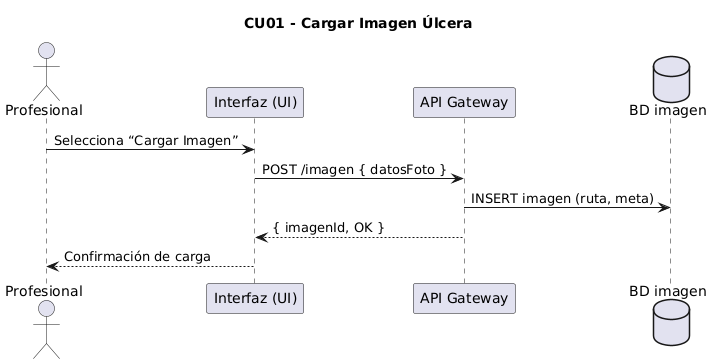
\includegraphics[width=0.8\textwidth]{imagenes/cu01_seq.png}
  \caption{CU01 – Cargar Imagen Úlcera. El Profesional sube o captura la fotografía clínica y el sistema la persiste en la base de datos de imágenes.}
  \label{fig:cu01_seq}
\end{figure}

\begin{figure}[H]
  \centering
  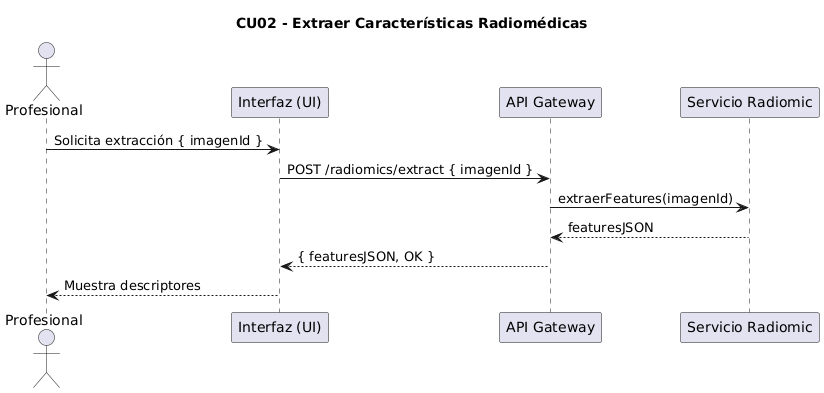
\includegraphics[width=0.8\textwidth]{imagenes/cu02_seq.png}
  \caption{CU02 – Extraer Características Radiomédicas. Después de la carga, el Profesional solicita el cálculo de descriptores radiómicos y el servicio asociado retorna los resultados.}
  \label{fig:cu02_seq}
\end{figure}

\begin{figure}[H]
  \centering
  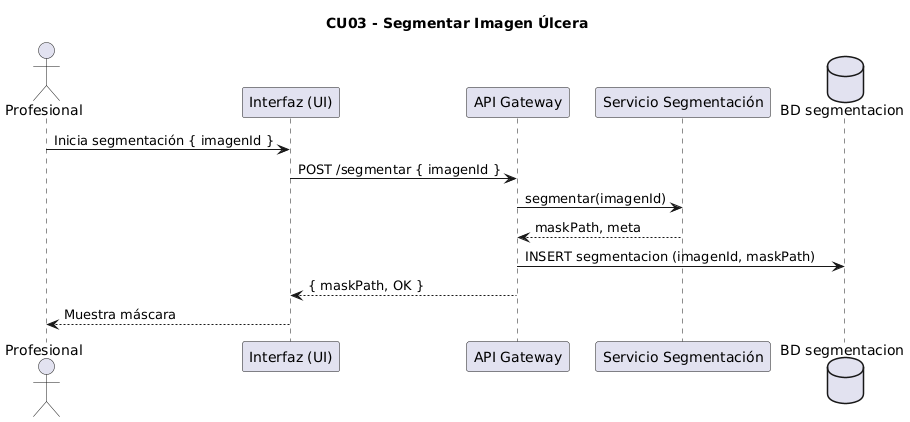
\includegraphics[width=0.8\textwidth]{imagenes/cu03_seq.png}
  \caption{CU03 – Segmentar Imagen Úlcera. El Profesional invoca la segmentación automática, que produce la(s) máscara(s) de herida y tejidos.}
  \label{fig:cu03_seq}
\end{figure}

\begin{figure}[H]
  \centering
  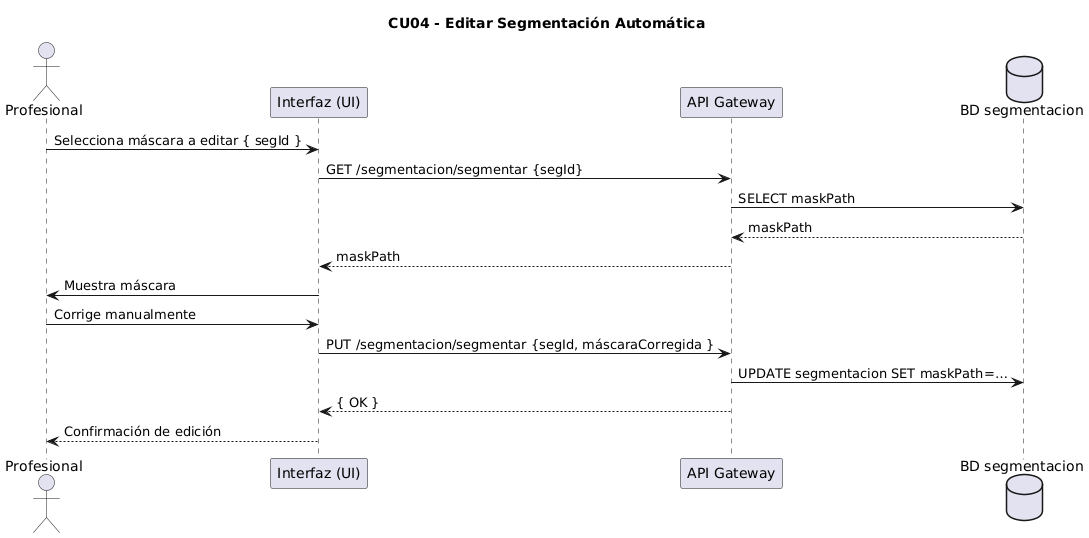
\includegraphics[width=0.8\textwidth]{imagenes/cu04_seq.png}
  \caption{CU04 – Editar Segmentación Automática. El Profesional corrige manualmente la máscara generada y almacena la versión ajustada.}
  \label{fig:cu04_seq}
\end{figure}

\begin{figure}[H]
  \centering
  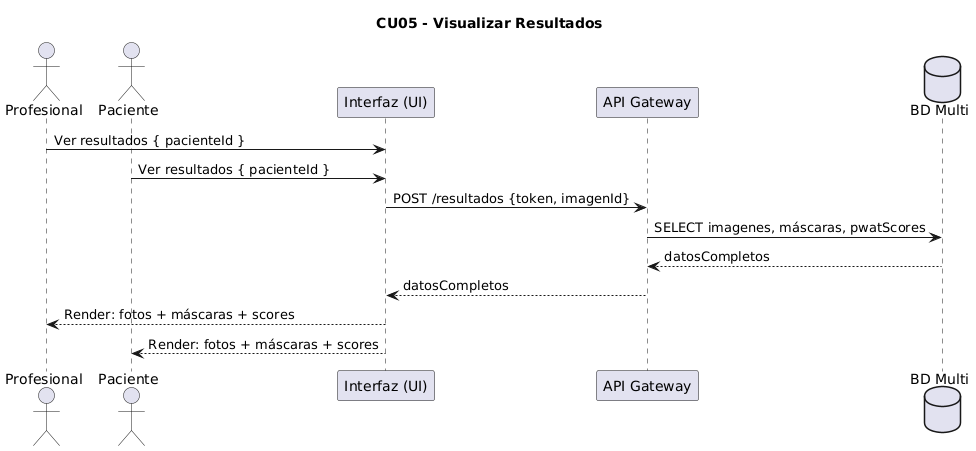
\includegraphics[width=0.8\textwidth]{imagenes/cu05_seq.png}
  \caption{CU05 – Visualizar Resultados. Profesional o Paciente recuperan y muestran la imagen, las máscaras y los puntajes PWAT generados.}
  \label{fig:cu05_seq}
\end{figure}

\begin{figure}[H]
  \centering
  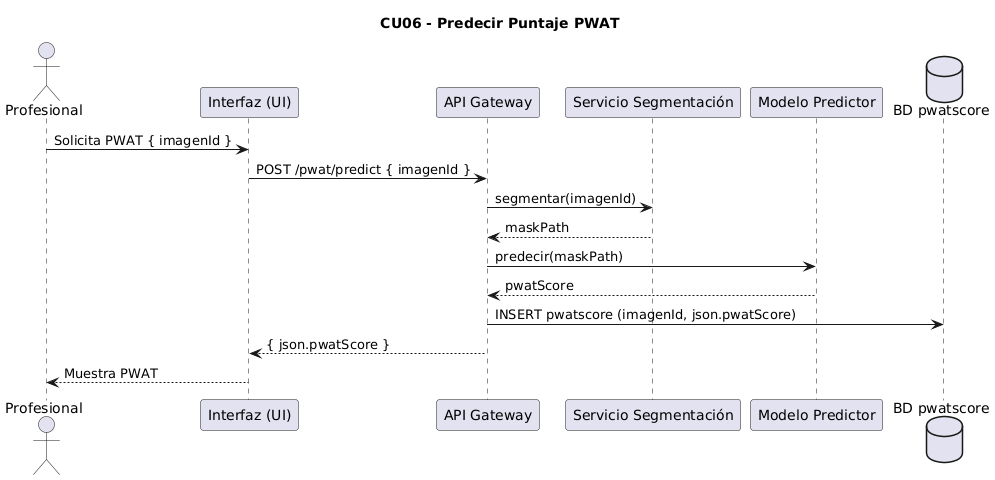
\includegraphics[width=0.8\textwidth]{imagenes/cu06_seq.png}
  \caption{CU06 – Predecir Puntaje PWAT. El Profesional solicita la predicción, se segmenta internamente y el Modelo Predictor devuelve el puntaje, que se guarda en la BD.}
  \label{fig:cu06_seq}
\end{figure}

\begin{figure}[H]
  \centering
  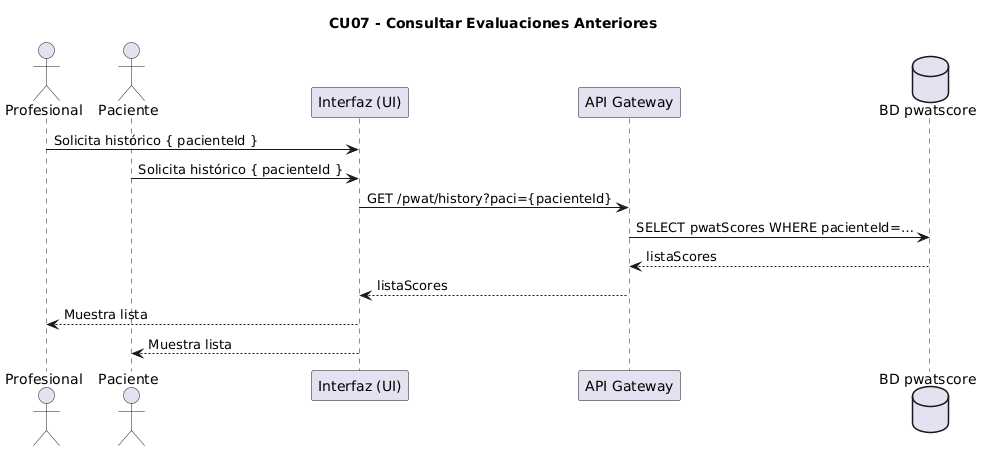
\includegraphics[width=0.8\textwidth]{imagenes/cu07_seq.png}
  \caption{CU07 – Consultar Evaluaciones Anteriores. Profesional o Paciente consultan el histórico de puntajes PWAT filtrados por paciente o imagen.}
  \label{fig:cu07_seq}
\end{figure}

\begin{figure}[H]
  \centering
  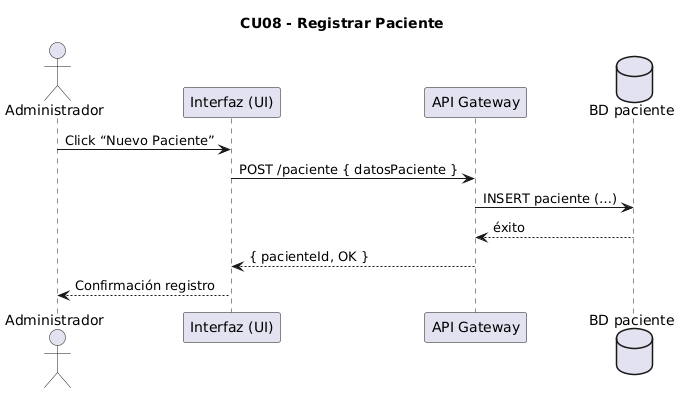
\includegraphics[width=0.8\textwidth]{imagenes/cu08_seq.png}
  \caption{CU08 – Registrar Paciente. El Administrador crea o actualiza registros en la tabla \texttt{paciente} mediante la interfaz.}
  \label{fig:cu08_seq}
\end{figure}

\begin{figure}[H]
  \centering
  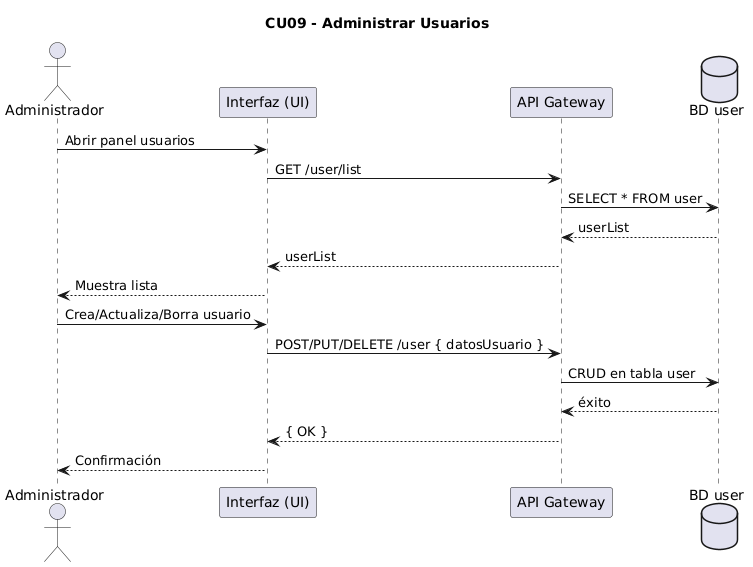
\includegraphics[width=0.8\textwidth]{imagenes/cu09_seq.png}
  \caption{CU09 – Administrar Usuarios. El Administrador realiza operaciones CRUD sobre la tabla \texttt{user}.}
  \label{fig:cu09_seq}
\end{figure}

\begin{figure}[H]
  \centering
  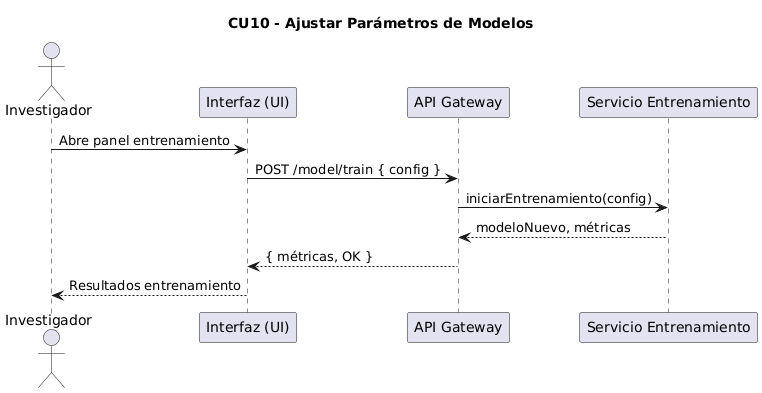
\includegraphics[width=0.8\textwidth]{imagenes/cu10_seq.png}
  \caption{CU10 – Ajustar Parámetros de Modelos. El Investigador lanza un nuevo entrenamiento o ajuste de hiperparámetros y recibe métricas.}
  \label{fig:cu10_seq}
\end{figure}

\begin{figure}[H]
  \centering
  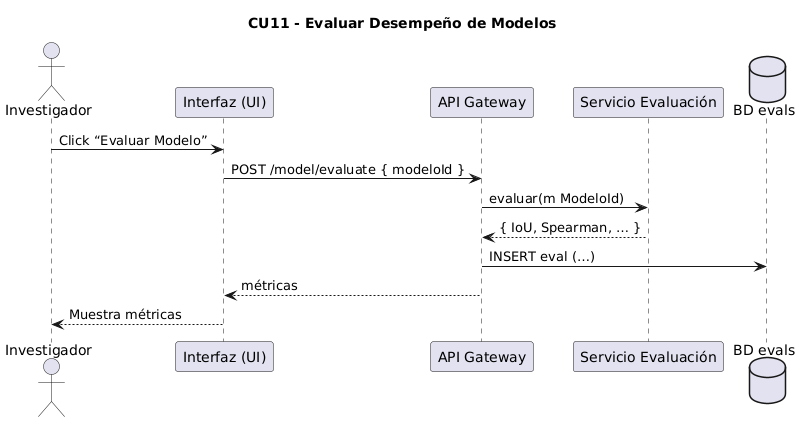
\includegraphics[width=0.8\textwidth]{imagenes/cu11_seq.png}
  \caption{CU11 – Evaluar Desempeño de Modelos. El Investigador solicita evaluación sobre test‐set y el sistema retorna métricas (IoU, Spearman, etc.).}
  \label{fig:cu11_seq}
\end{figure}

\subsection{Diagramas de Estado}
\label{ssc:DE}

A continuación se presentan los diagramas de estado para los tres elementos clave del sistema: \texttt{Imagen}, \texttt{Segmentación} y \texttt{PwatScore}. Cada figura muestra los estados por los que atraviesa el objeto y las transiciones disparadas por los casos de uso correspondientes.

\begin{figure}[H]
  \centering
  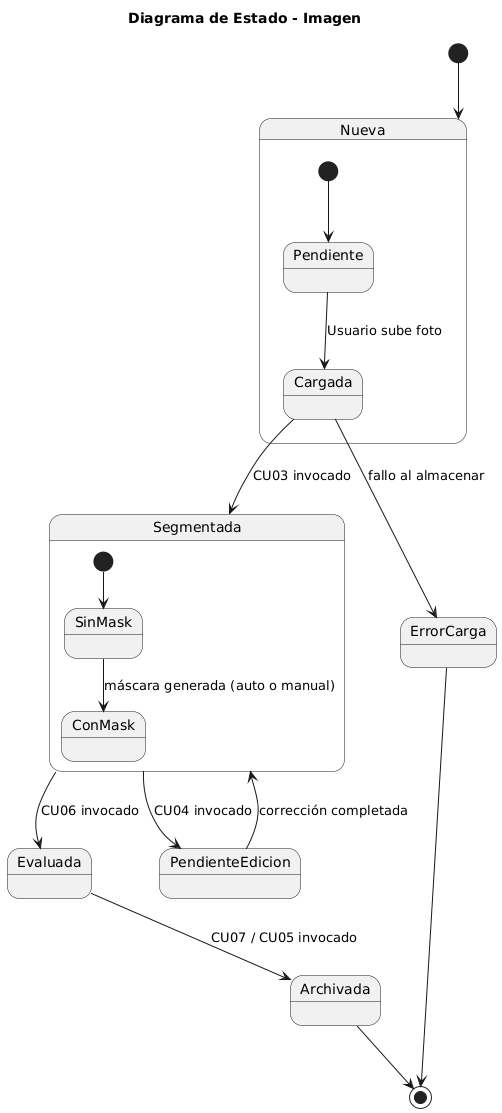
\includegraphics[width=0.95\textwidth,height=0.5\textheight,keepaspectratio]{imagenes/estado_imagen.png}
  \caption{Diagrama de estado de la entidad \texttt{Imagen}.}
  \label{fig:estado_imagen}
\end{figure}

\begin{figure}[H]
  \centering
  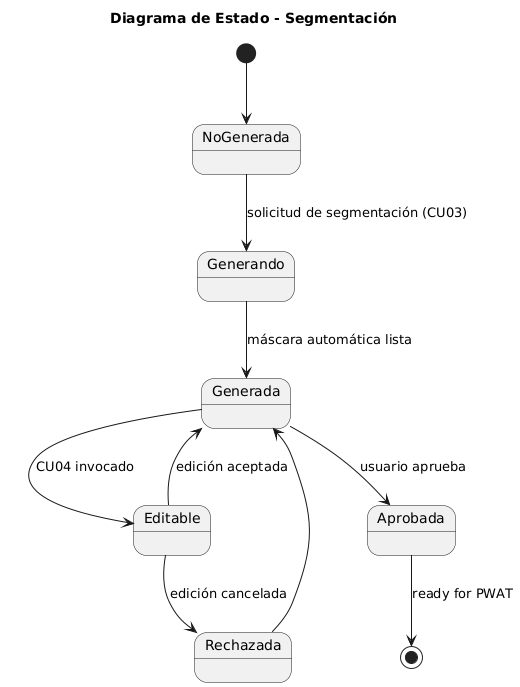
\includegraphics[width=0.95\textwidth,height=0.5\textheight,keepaspectratio]{imagenes/estado_segmentacion.png}
  \caption{Diagrama de estado de la entidad \texttt{Segmentación}.}
  \label{fig:estado_segmentacion}
\end{figure}

\begin{figure}[H]
  \centering
  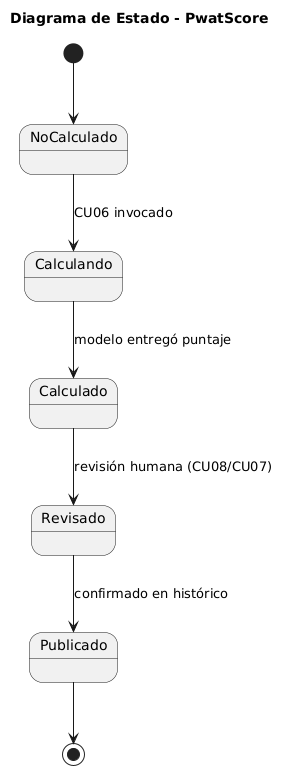
\includegraphics[width=0.95\textwidth,height=0.5\textheight,keepaspectratio]{imagenes/estado_pwatscore.png}
  \caption{Diagrama de estado de la entidad \texttt{PwatScore}.}
  \label{fig:estado_pwatscore}
\end{figure}

\subsection{Modelo Conceptual}
\label{ssc:MC}

A continuación se describe el modelo conceptual (diagrama de entidades y relaciones) que organiza las principales entidades del sistema y sus interacciones:

\begin{itemize}
  \item \textbf{User}: representa a todos los usuarios de la plataforma (clínicos, administradores e investigadores). Contiene atributos de identificación, datos de contacto y rol.
  \item \textbf{Profesional}: extiende a \texttt{User} con la especialidad y vincula al médico o enfermero responsable de pacientes.
  \item \textbf{Paciente}: almacena la información demográfica y clínica básica, referenciando al \texttt{User} que lo registró y al \texttt{Profesional} asignado.
  \item \textbf{Imagen}: guarda cada fotografía de la úlcera (nombre, fecha, ruta) asociada a un \texttt{Paciente}.
  \item \textbf{Segmentación}: registra cada máscara (método, ruta, fecha) aplicada sobre una \texttt{Imagen}, ya sea manual o automática.
  \item \textbf{PWATScore}: conserva los puntajes PWAT (valor numérico, evaluador, detalles en JSON, fecha), referenciando tanto la \texttt{Imagen} como la \texttt{Segmentación} empleada.
\end{itemize}

Las relaciones principales son:
\begin{itemize}
  \item Un \texttt{User} puede registrar múltiples \texttt{Profesional} y \texttt{Paciente}.
  \item Un \texttt{Profesional} está a cargo de cero o más \texttt{Paciente}.
  \item Cada \texttt{Paciente} puede tener varias \texttt{Imagen}, y cada \texttt{Imagen} puede generar múltiples \texttt{Segmentación} y \texttt{PWATScore}.
  \item Cada \texttt{Segmentación} está vinculada a una única \texttt{Imagen}, y cada \texttt{PWATScore} se apoya en una \texttt{Imagen} y una \texttt{Segmentación}.
\end{itemize}

Este esquema asegura la trazabilidad completa desde el registro de usuarios y pacientes, pasando por la captura y segmentación de imágenes, hasta la evaluación cuantitativa del estadio de la herida mediante puntajes PWAT.

\begin{figure}[H]
  \centering
  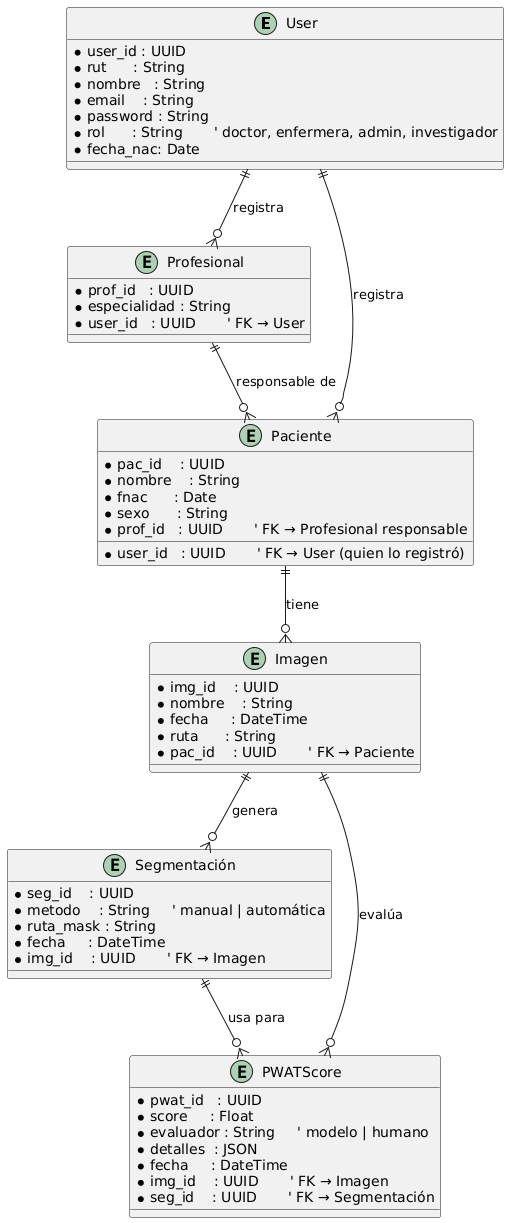
\includegraphics[
    width=\textwidth,
    height=0.9\textheight,
    keepaspectratio
  ]{imagenes/modelo_conceptual.png}
  \caption{Diagrama conceptual de entidades y relaciones del sistema.}
  \label{fig:modelo_conceptual}
\end{figure}
